\documentclass[14pt, a4paper]{extarticle}
\usepackage[14pt]{extsizes}
\usepackage[utf8]{inputenc}
\usepackage[russian]{babel}
\usepackage{amsmath}
\usepackage{amsfonts}
\usepackage{graphicx}
\usepackage{amssymb}
\usepackage[left=2cm,right=2cm,top=2cm,bottom=2cm,bindingoffset=0cm]{geometry}
\usepackage{graphicx}
\usepackage[T2A]{fontenc} 
\usepackage{multicol}
\usepackage{caption}
%\usepackage{subcaption}
\usepackage{textcomp} 
\usepackage{setspace} 
\usepackage{chngcntr}
\usepackage[small]{titlesec} 
\setlength{\parindent}{1.25cm}
\renewcommand{\baselinestretch}{1.3}
\usepackage{cmap}
\AtBeginDocument{\let\textlabel\label}
\usepackage{hyperref}
\hypersetup{pdftex,colorlinks=true,linkcolor = black, citecolor = blue, backref=page}
\usepackage[all]{hypcap}

\usepackage{subfig}
\graphicspath{ {img/} }

%\bibliographystyle{gost780u}
\bibliographystyle{unsrt}

%\counterwithin{equation}{section}
\renewcommand{\theequation}{\arabic{section}.\arabic{subsection}.\arabic{equation}}
\newcommand{\RNumb}[1]{\uppercase\expandafter{\romannumeral #1\relax}}
\begin{document}
	\begin{titlepage}
		\begin{center}
			\hfill \break
			МОСКОВСКИЙ ФИЗИКО-ТЕХНИЧЕСКИЙ ИНСТИТУТ\\ (ГОСУДАРСТВЕННЫЙ УНИВЕРСИТЕТ)\\
			\hfill \break
			\hfill \break
			\hfill \break
			\hfill \break
			\hfill \break
			Департамент философии\\
			\hfill \break
			\hfill \break
			РЕФЕРАТ ПО ИСТОРИИ НАУКИ\\
			\hfill \break
			\hfill \break
			\large{\textbf{ИСТОРИЯ РАЗВИТИЯ И ПРОБЛЕМЫ БИОМЕТРИЧЕСКОГО РАСПОЗНАВАНИЯ ЧЕЛОВЕКА}}\\
			\hfill \break		
		\end{center}
		
		\begin{center}
			\hfill \break
			\parbox{0.9\textwidth}
			{
				Аспирант~--- Соломатин Иван Андреевич \\
				Научный руководитель аспиранта \underline{\hspace{3cm}} д.т.н. Матвеев И.А. \\
				Преподаватель департамента философии~--- Фурсов А.А. \\
			}
		\end{center}
		\hfill \break
		\hfill \break
		\hfill \break
		\hfill \break
		\begin{center} Москва, 2018 
		\end{center}
		\thispagestyle{empty} 
	\end{titlepage}
	
\tableofcontents
\newpage

\section{Введение}
На протяжении всей истории человечества задача распознавания человека была актуальной, однако в последние годы интерес к ней многократно возрос. В основном, это вызвано появлением новых технических средств и всё более глубоким их проникновением в повседневную жизнь людей. Набор технических приёмов, применяемых для распознавания человека по физическим и поведенческим параметрам в наше время принято называть \textit{биометрией}. Появившиеся технические возможности открывают новые методики и совершенно новые и неожиданные сферы применения биометрии. В современном виде биометрия стала применяться с конца \texttt{XIX} века в криминалистике и применяется в этой области до сих пор \cite{tistarelli2014biometrics, bouchrika2011using}. В настоящее время слово "биометрия"\ у всех на слуху: биометрическое распознавание используется в смартфонах \cite{odinokikh2018high, sezan2014user, hwang2009keystroke}, в банковском деле \cite{fatima2011banking, venkatraman2008biometrics}, в маркетинге, в социологии (в сфере социального управления).

Сама постановка задачи распознавания человека по каким-либо признакам имеет глубокие корни, уходящие далеко в прошлое. На самом деле, любой человек, не задумываясь, решает эту задачу каждый день по многу раз, когда узнаёт своих родных, друзей, коллег. Чаще всего, при социальном взаимодействии, человек выстраивает диалог и предпринимает те или иные действия, исходя из знания того, с кем именно он взаимодействует. Таким образом, данная задача лежит в основе социального взаимодействия людей, и именно поэтому она настолько актуальна и обсуждаема.

В данной работе описывается история развития различных систем распознавания, а также некоторые проблемы и вызовы, связанные с подобными системами.

\newpage
\section{Постановка задачи распознавания человека}
Под термином "распознавание человека"\ можно понимать две принципиально разные задачи~--- задачу идентификации, и задачу аутентификации. 


В общем виде постановку этих задач можно сформулировать следующим образом. \\
\textbf{Задача аутентификации}. Необходимо:
\begin{itemize}
	\item Считать с человека биометрические данные с помощью какого-либо устройства;
	\item Обработать полученные данные, получив некоторый биометрический идентификатор человека (биометрический шаблон);
	\item Сравнить полученный шаблон с шаблоном, или шаблонами из базы данных, которые соответствуют одному человеку, и сказать, являются ли эти два объекта (человек, с которого был получен текущий шаблон, и человек, с которого был получен шаблон из базы) одним и тем же человеком или разными.
\end{itemize}

Другими словами, аутентификация~--- это проверка, что исследуемый человек является именно тем, за кого он себя выдаёт.

В постановке задачи идентификации первые два пункта аналогичны пунктам для аутентификации. Отличается лишь третий пункт.\\
\textbf{Задача идентификации}. Необходимо:
\begin{itemize}
	\item Считать с человека биометрические даннные;
	\item Обработать полученные данные, получив биометрический шаблон;
	\item Сравнить полученный шаблон с \textit{каждым} шаблоном из базы данных и сказать, кем является исследуемый человек, или, что соответствующего ему шаблона нет в базе.
\end{itemize}

Другими словами, идентификация~--- это проверка, кем именно является исследуемый человек.

Эти формулировки задач достаточно обобщённые, и для более точной постановки задачи нужно уточнить, какие биометрические данные будут считываться с человека, какое устройство будет для этого использовано, какие алгоритмы будут использоваться для получения и сравнения биометрических шаблонов. 

\newpage
\section{История развития систем распознавания человека}
Как было сказано выше, задача распознавания человека была актуальной испокон веков. До появления науки биометрии людям тоже нужно было идентифицировать себя и подтверждать (аутентифицировать) свою личность. Для этого изобретались различные устройства и системы.
Например, для подтверждения авторства писем ещё в конце \texttt{IV} века в Риме начали использовать сургучные печати. Печати используются для подтверждения подлинности документов и по сей день.

Больший же интерес для данной работы представляют системы именно биометрического распознавания, то есть распознавания по физическим и поведенческим параметрам. Существует множество параметров, по которым можно построить систему биометрического распознавания человека, такие параметры называются \textit{биометрическими модальностями}. И, как следствие, существует множество разновидностей таких систем. Ниже описывается история развития систем распознавания по основным биометрическим модальностям, которые активно используются в наше время или активно использовались в прошлом.

\subsection{Бертильонаж}
Бертильонаж~--- система идентификации человека по антропометрическим данным. Названа в честь своего изобретателя~--- Альфонса Бертиль\'{о}на.

Работая писарем в полиции Парижа и переписывая карточки с описанием преступников, Альфонс Бертильон обратил внимание на то, что данные описания являются крайне поверхностными и нечёткими, например, "высокого роста"\ , "плотного телосложения"\  и т.п. Бертильон предложил использовать для идентификации преступников точные измерения различных частей тела. Проведя серию экспериментов, он предложил использовать для этого метода следующие параметры: длина головы, ширина головы, длина среднего пальца, длина левой ступни и длина локтя \cite{bertillon}. Впервые система была успешно использована создателем 20 февраля 1883 года, когда он опознал в одном из заключённых преступника, который уже был осуждён ранее и измерен. Но по-настоящему большую известность система получила 30 марта 1892, когда с её помощью удалось обнаружить и арестовать организатора серии террористических актов в Париже.
Система с успехом применялась Французской полицией до 1914 года~--- года смерти Бертильона. После его смерти место бертильонажа заняла дактилоскопия, или распознавание по отпечаткам пальцев.
\subsection{Распознавание по отпечаткам пальцев}
Распознавание по отпечаткам пальцев~--- первая научно обоснованная методика биометрического распознавания. Она основана на уникальности рисунка на пальцах человека, называемого папиллярным узором. На рис. \ref{img:fingerprints} изображены примеры этих узоров.

\begin{center}
	\begin{figure}[h!]
		\centering
		\subfloat[Петля]{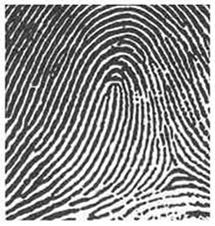
\includegraphics[width=0.25\textwidth]{fingerprint_1.png}}
		\hspace{0.05\textwidth}
		\subfloat[Дуга]{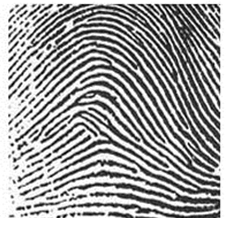
\includegraphics[width=0.25\textwidth]{fingerprint_2.png}}
		\hspace{0.05\textwidth}
		\subfloat[Завиток]{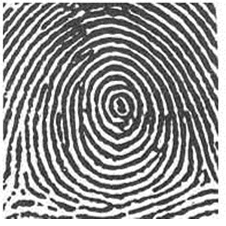
\includegraphics[width=0.25\textwidth]{fingerprint_3.png}}
		\caption{Примеры папиллярных узоров различных типов}
		\label{img:fingerprints}
	\end{figure}
\end{center}

\vspace{-1cm}

Первое упоминание об использовании отпечатков пальцев относится к древним временам. Уже в древнем Вавилоне и древнем Китае люди использовали эти уникальные узоры для подписи документов. Кроме того, согласно работе \cite{xiang1988historical}, историки нашли свидетельство того, что в Китае уже в конце \texttt{III} века до нашей эры отпечатки пальцев использовались в криминалистике для идентификации преступников. 

Впервые папиллярные узоры на пальцах человека были описаны итальянским биологом и врачом Марчелло Мальпиги в его работе \cite{malpighi1669opera}, датированной 1669 годом. Первое упоминание о том, что рисунок папиллярных линий пальца является уникальным для каждого человека, принадлежит Иоганну Кристофу Андреасу Майеру, который написал об этом в своей работе по анатомии \cite{mayer1794anatomische}, опубликованной в 1794 году. 

В 1823 году чешский учёный Ян Эвангелиста Пуркинье опубликовал работу \cite{purkynve2013dissertation}, в которой впервые предлагалась классификация папиллярных узоров, содержащая девять основных типов узоров, которая заложила фундамент современной дактилоскопии. 

Одним из основоположников дактилоскопии является Уильям Хершел, который доказал, что узор на пальцах не меняется на протяжении жизни человека, а также после его смерти. С 1858 года Хершел, работавший чиновником в Индии, начал использовать отпечатки пальцев для подтверждения подлинности документов. В 1877 г. он предложил использовать отпечатки пальцев для регистрации заключённых. Это был первый случай научно обоснованного практического использования дактилоскопии.

В наше время существует множество алгоритмов, позволяющих распознавать человека по отпечатку пальца в автоматическом режиме. Такие алгоритмы используются как в криминалистике, так и в повседневной жизни людей: в большинстве смартфонов, в персональных компьютерах, биометрических замках, и т.д.

\subsection{Распознавание по радужной оболочке глаза}
Радужка~--- передний отдел сосудистой оболочки глазного яблока, видимый через прозрачную роговицу \cite{petrovskiy1974bme}. Радужка имеет яркую окраску и обладает слабо меняющейся со временем структурой, которая содержит в себе одни из наиболее надёжных признаков для распознавания человека. Регистрацию изображения радужной оболочки можно произвести дистанционно и неинвазивно, с использованием неслепящей направленной подсветки. Данная биометрическая модальность считается самой эффективной на данном этапе развития биометрии \cite{gupta2011iris}.

Первое упоминание об использовании радужной оболочки для распознавания личности принадлежит глазному хирургу Франкe Буршe, и было сделано в 1936 году \cite{misztal2012iris}.


\begin{center}
\begin{figure}[h!]
	\centering
	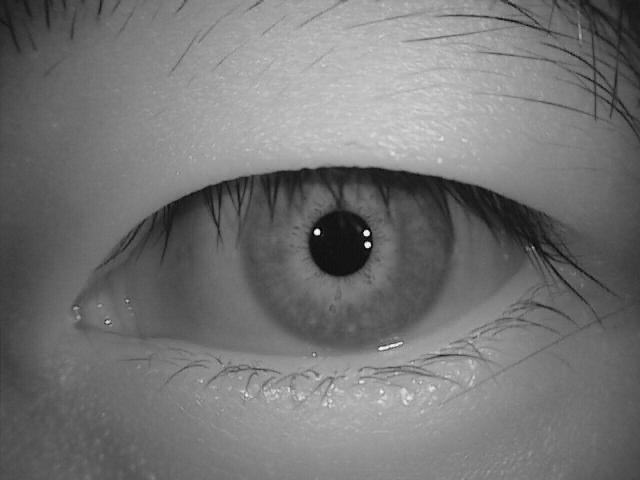
\includegraphics[width=0.45\textwidth]{iris_sample_1.png}
	\hspace{0.05\textwidth}
	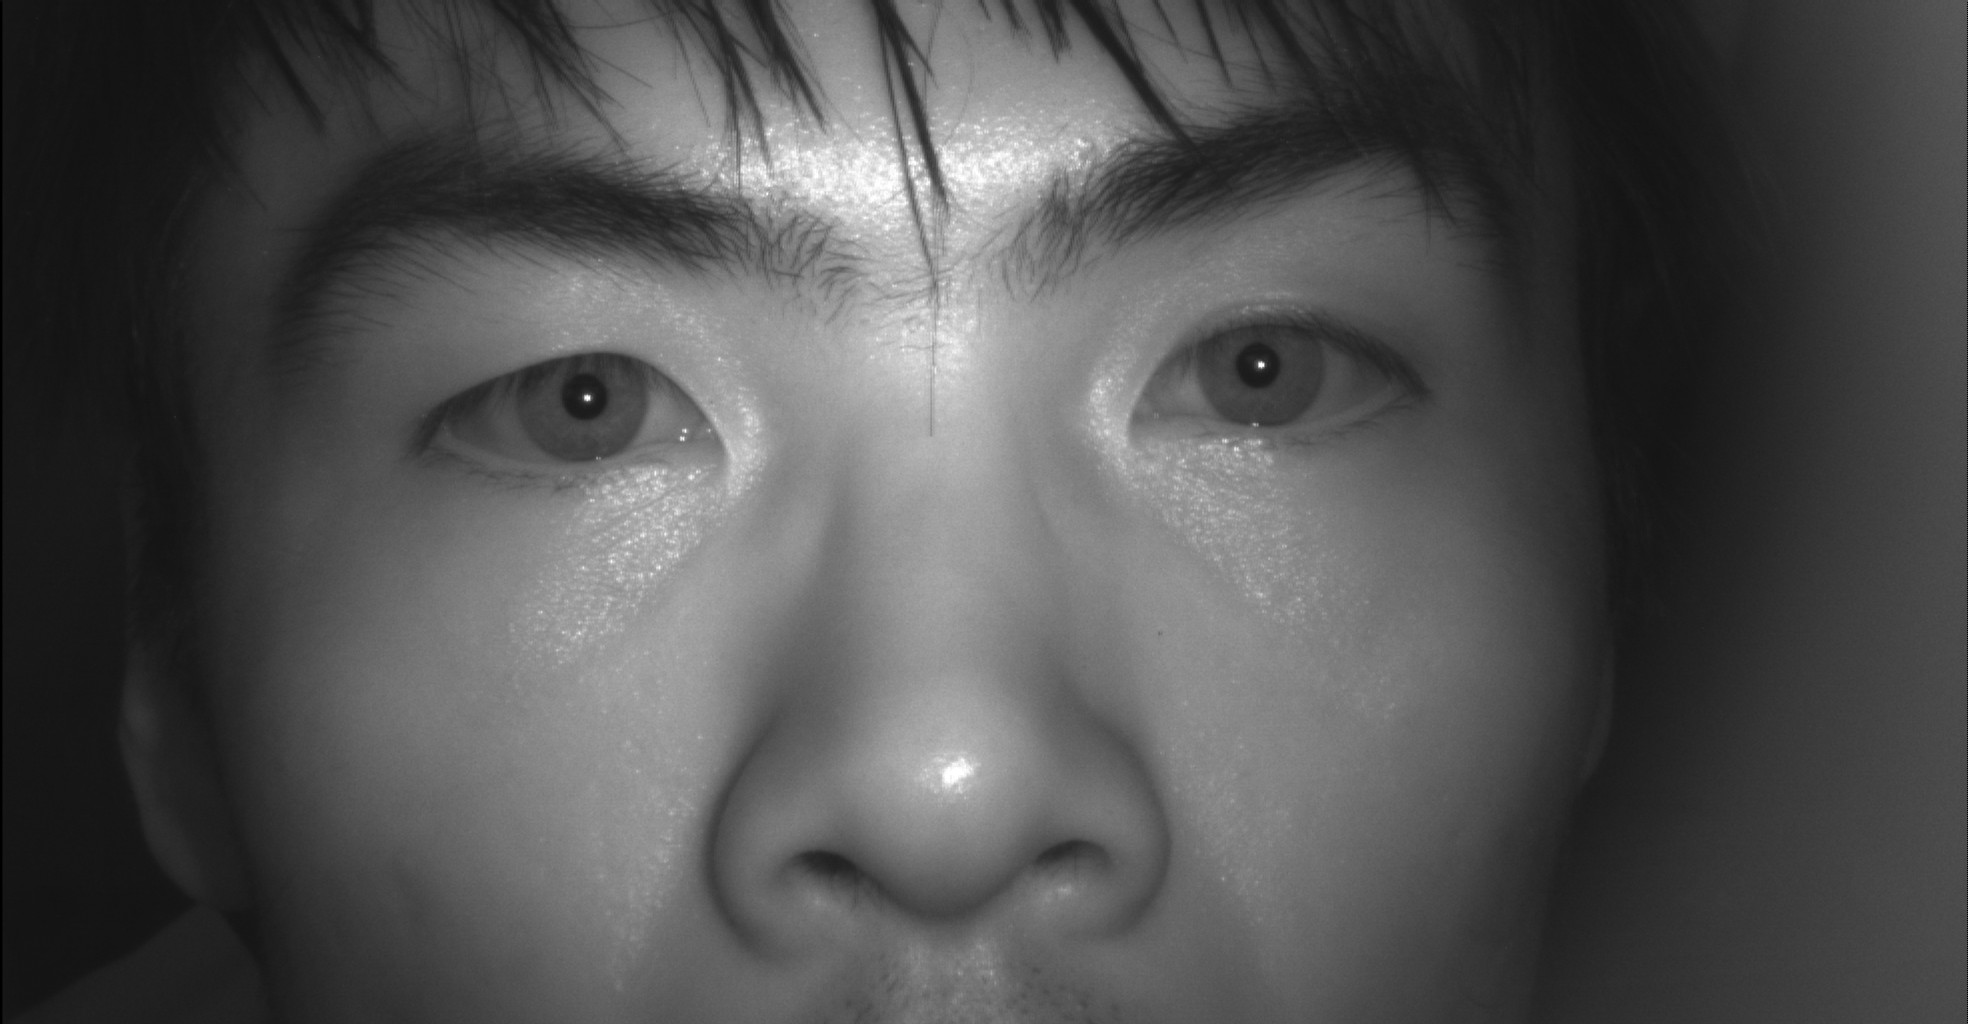
\includegraphics[width=0.45\textwidth]{iris_sample_2.png}
	\caption{Примеры изображений, используемых для распознавания человека по радужной оболочке.}
	\label{img:iris_samples}
\end{figure}
\vspace{-1cm}
\end{center}

На основе его исследований офтальмологи Л. Флом и А. Сафир в 1987 г. запатентовали основные принципы распознавания по радужной оболочке \cite{flom1987iris}. Для разработки алгоритма А. Сафир и Л. Флом обратились за помощью к Джону Даугману, который, впоследствии, в 1994 г. запатентовал первую систему идентификации личности по изображению радужки \cite{daugman1994biometric}, и считается родоначальником этого вида распознавания. Основными этапами работы алгоритма, запатентованного Даугманом являются сегментация радужки, выделение признаков в этой области, их кодирование и классификация.
Большинство систем распознавания по радужной оболочке используют изображения, полученные в ближнем инфракрасном диапазоне, поскольку радужная оболочка в этом случае содержит меньшее количество бликов и имеет более контрастную структуру \cite{Daugman02}. Примеры изображений радужной оболочки приведены на рис. \ref{img:iris_samples}.

В последнее время алгоритм Даугмана начинает постепенно уступать в скорости и точности распознавания новым алгоритмам, которые используют искуственные нейронные сети.

В настоящее время распознавание по радужной оболочке используется в мобильных устройствах \cite{odinokikh2018high}, в биометрических замках и в различных системах контроля доступа.

\subsection{Распознавание по лицу}
Распознавание человека по лицу~--- самый естественный метод биометрического распознавания, поскольку именно так мы привыкли узнавать друг друга в повседневной жизни. История изучения этой биометрической модальности, в отличие, например, от отпечатков пальцев, началась только с появлением ЭВМ. До появления ЭВМ узнать человека по фотографии или рисунку не составляло особого труда, поскольку любой человек умеет это делать от природы, и ему не требуются для этого какие-то алгоримы, но, с появлением ЭВМ, возник вопрос: как научить компьютер распознавать лица? Именно в направлении ответа на этот вопрос и велись исследования в области данной биометрической модальности.

Первой системой распознавания лиц была система \cite{bledsoe1968face}, разработанная в 1968 году Вудро Бледсоу, американским учёным в области искусственного интеллекта. Система была полуавтоматической, то есть требовала участия человека. При пользовании этой системой человек должен был вручную отмечать отличительные характеристики лица на фотографии. Скорость обработки с помощью данной системы составляла около 40 лиц в час.

В задаче автоматического распознавания человека по лицу выделяют три основные задачи:
\begin{enumerate}
	\item Обнаружение и грубая нормализация лица на изображении;
	\item Выделение ключевых точек и других необходимых параметров и более точная нормализация лица;
	\item Идентификация, аутентификация.
\end{enumerate}

Дальнейшие исследования в области распознавания человека по лицу велись и до сих пор ведутся в направлении улучшения точности решения каждой из этих подзадач и уменьшения ограничений на входные данные. Например, первые системы распознавания требовали чётко выверенного положения лица на фотографии, однотонный фон, равномерное освещение. Современные системы всё более и более приближаются к человеческим способностям в области распознавания лиц, а во многом уже даже превосходят человека.

В последнее время всё большей популярностью пользуются алгоритмы распознавания человека по 3D отпечатку лица \cite{paysan20093d}. Преимущество данного метода состоит в том, что 3D отпечаток несёт в себе гораздо больше информации, чем простая фотография, а значит, и точность такого распознавания выше.

В наше время распознавание лиц используется в смартфонах, в банковском деле и является очень популярным, поскольку метод получения данных для данной биометрической модальности очень прост~--- нужна только фотография лица. Простота получения данных влечёт за собой удобство, так как для использования системы распознавания не требуется дополнительных условий или действий.

\subsection{Распознавание по голосу}
Голос и речь человека имеет ряд специфических особенностей, что позволяет нам безошибочно узнавать знакомых даже не видя их. Мы подсознательно выделяем ряд параметров и характеристик, которые могут быть технически зафиксированы и подвергнуты анализу.

Распознавание человека по голосу идёт рука об руку с распознаванием речи человека. Первые успешные эксперименты по распознаванию человеческой речи были сделаны в 50-х годах XX века в корпорации Bell Laboratories в США. Тогда удалось добиться устойчивого распознавания цифр, произносимых человеком, на которого была настроена система. К началу 60-х годов технология позволила распознавать некоторые гласные буквы, произносимые разными людьми и различать людей, произносящих эти гласные буквы. Задачи распознавания речи и распознавания говорящих людей развивались паралельно. К началу 90-х с появлением методов искусственных нейронных сетей были достигнуты прорывные результаты и появились устройства, которые начали применяться в реальной жизни. Наиболее интенсивно развивалось применение голосовой идентификации в криминалистике и в сфере банковских услуг. 

Сейчас некоторые банковские контакт-центры успешно применяют голосовые технологии. При обращении в банк по телефону, голос клиента автоматически фиксируется и анализируется, и если он хочет совершить какую-то операцию, для которой требуется аутентификация, то его личность проверяется по его голосу. При этом клиенту даже не требуется называть никаких паролей. Первым объявил о доступности такой технологии британский банк HSBC. 

В криминалистике задача, как правило, состоит в том, чтобы, имея запись речи, установить принадлежит ли голос на записи человеку, образец голоса которого доступен. Подобный анализ называется «Фоноскопическая экспертиза» и применяется достаточно давно. В нашей стране в середине 90-х годов был внедрён аппаратно-программный комплекс «Диалект», который успешно применялся в Министерстве Внутренних дел.

%Одни из самых известных производителей на рынке голосовой биометрии — Nuance Communications (ранее компания называлась SpeechWorks)

Главным достоинством голосовой идентификации является высокая устойчивость к фальсификации. Человек может очень точно копировать чужую речь, настолько точно, что окружающие люди не смогут ощутить подделку, но основные параметры, на которые опираются современные системы голосового распознавания, не доступны уху подражателя и окружающих, поэтому подделать их человек не может. При этом машинные алгоритмы синтеза речи развиваются бурными темпами. В 2018 году сразу две компании объявили о создании систем копирования речи людей. Китайские специалисты из компании Baidu создали нейросеть под названием Deep Voice, другая нейронная сеть имеет название Lyrebird и разработана одноимённой канадской компанией. Разработчики и того, и другого решения утверждают, что их системы, прослушивая голос человека в течение короткого промежутка времени, обучаются его имитировать. При этом точность имитации такова, что люди не могут отличить подделку. Вполне возможно, что столкновение зеркальных технологий~--- идентификации человека по голосу и имитации голоса человека превратится в новое соревнование брони и снаряда. Что, конечно, является потенциальным недостатком идентификации человека по голосу. Вторым недостатком всегда была чувствительность к естественному изменению голоса в результате болезней и старения человека. 
\subsection{Распознавание по походке}
Большая медицинская энциклопедия определяет походку как "совокупность признаков, характеризующих ходьбу человека. Ряд двигательных компонентов походки имеет врожденный характер и включен в сложную координированную деятельность мышц и конечностей в процессе передвижения."\ \cite{petrovskiy1974bme} Походка отражает личностные особенности человека (характер, темперамент), что делает её совершенно уникальной. Для получения биометрических данных используются специальные платформы, фиксирующие положение и динамические параметры подошв обуви при прохождении по ним людей, или тоннели с многочисленными видеокамерами, которые позволяют создать 3D модель перемещения ключевых точек человеческого скелета.

\begin{center}
	\begin{figure}[h!]
		\centering
		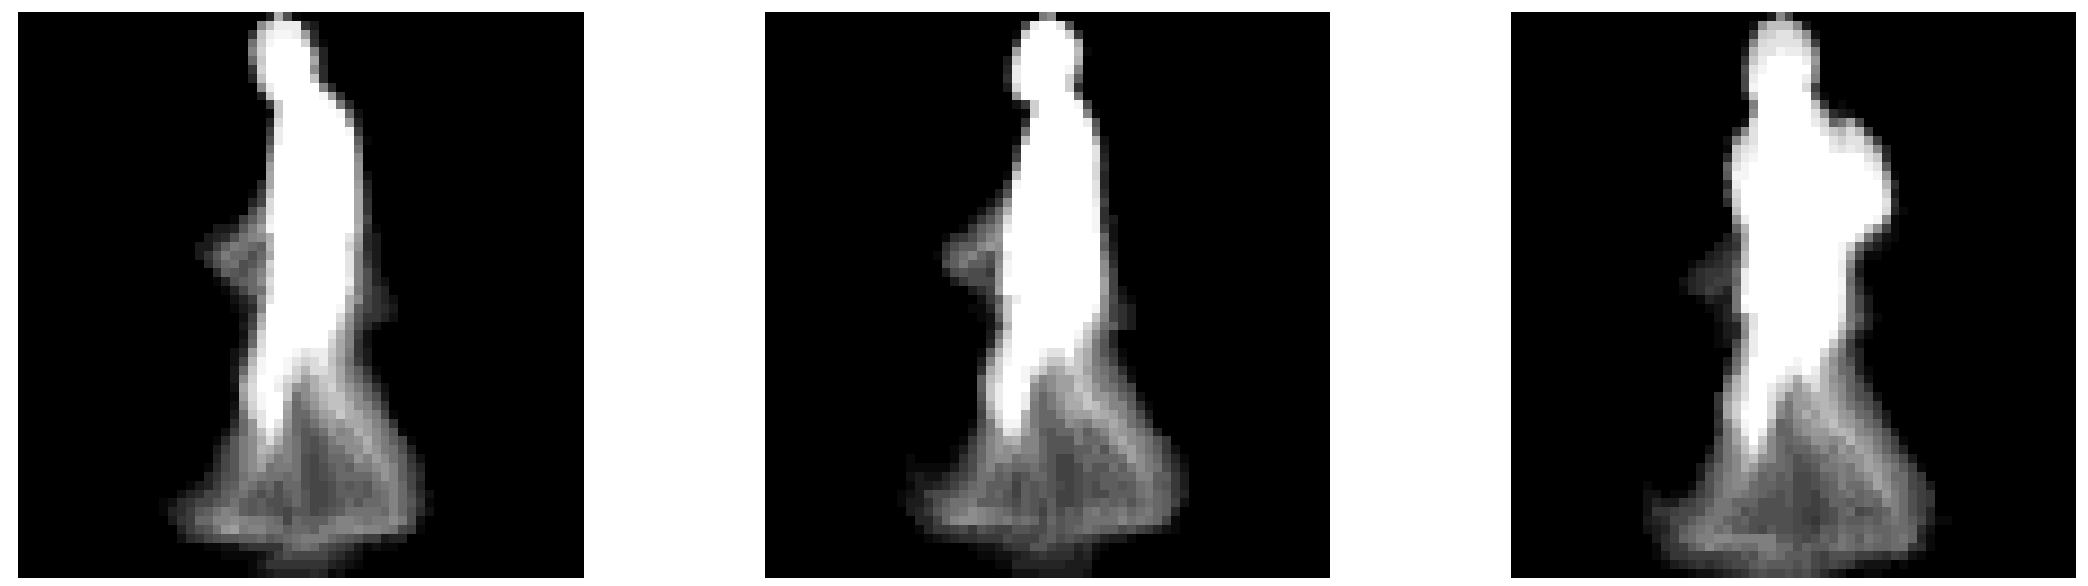
\includegraphics[width=0.7\textwidth]{gate.PNG}
		\caption{Примеры кадров из видеопоследовательности, используемой для распознавания по походке \cite{veres2005fusion}.}
		\label{img:gate}
	\end{figure}
\end{center}
\vspace{-1cm}

На рис. \ref{img:gate} приведены примеры кадров из видеопоследовательности, используемой для распознавания по походке. 

Возрастающие возможности нейронных сетей резко повышают точность и доступность подобных систем. В ближайшее время их применение может стать массовым.
В настоящее время Китайские учёные ведут разработку системы, позволяющей узнать человека в толпе по видеокадрам с уличных камер наблюдения. 

Важным достоинством данной биометрической модальности является невозможность фальсификации данных. Нельзя научить одного человека ходить в точности так, как ходит другой человек.

Так же, привлекательность использования особенностей походки в целях идентификации человека обусловлена простотой, ненавязчивостью или даже скрытностью получения данных. От человека требуется просто пройти некоторое расстояние своей обычной походкой. Кроме того, походку тяжело скрыть, как, например, лицо, или глаза. Если человек идёт по улице, он демонстрирует свою походку, по которой может быть идентифицирован. Именно эта простота и скрытность вызвала интерес со стороны всевозможных служб безопасности, в первую очередь в аэропортах.
\subsection{Распознавание по форме ушной раковины}
Впервые использовать анатомические особенности уха для идентификации человека предложил Альфонс Бертильон в 80-х годах \texttt{XIX} века. Он использовал измерения уха в качестве одного из признаков, по которым проводилась идентификация в методе бертильяжа.

%В 1906 году пражский отоларинголог Р. Имхофер после обследования 500 пар ушей пришел к выводу, что их можно четко различать всего по четырем особенностям.

%Более чем 50 лет спустя команда исследователей изучила фотографии 200 пар ушей новорожденных и пришла к заключению, что благодаря анатомическому постоянству уха по нему можно устанавливать личность младенцев.

Важной вехой в исследовании данной биометрической модальности было исследование Альфреда Янарелли, который в период с 1948-го по 1962 год собрал фотографии ушей нескольких тысяч человек и на основе их анализа предложил набор из 12 геометрических измерений уха (рис. \ref{img:ear}). Он утверждал, что, используя этот набор измерений, можно достоверно идентифицировать человека, так как он является уникальным.

\begin{center}
	\begin{figure}[h!]
		\centering
		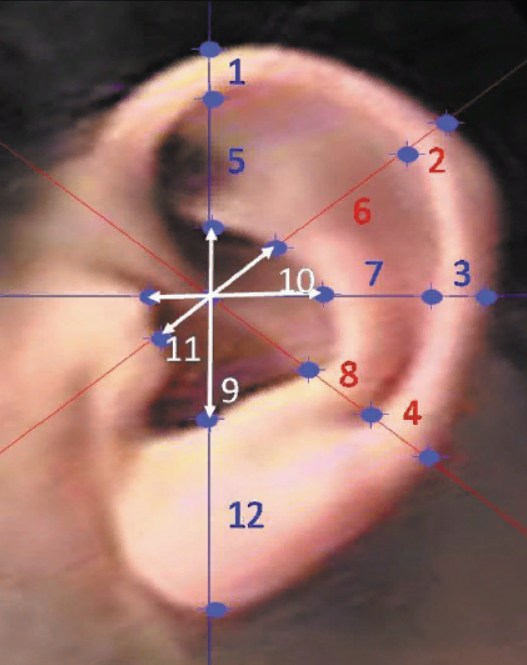
\includegraphics[width=0.4\textwidth]{ear.png}
		\caption{Набор из 12 геометрических измерений уха по А. Янарелли}
		\label{img:ear}
	\end{figure}
\end{center}
\vspace{-1cm}

В начале 2015 года в Yahoo Labs предложили идентифицировать владельца смартфона по его ушным раковинам. Предложенный алгоритм был назван Bodyprint, и описан в работе \cite{holz2015bodyprint}. Ученые предложили проводить верификацию владельца в момент соприкосновения уха с сенсорным экраном смартфона в процессе звонка. Точность биометрической идентификации данной системы по результатам тестирования составил 99,5\%. Инженеры Yahoo Labs предложили также модифицировать процедуру ответа на звонок: и инициировать начало разговора при соприкосновении смартфона с ухом вместо нажатия на кнопку приема.

\subsection{Тест ДНК}
Идентификация по ДНК~--- это установление генетической индивидуальности любого организма на основе анализа особенностей его ДНК. 

%В основе идентификации лежат две характеристики ДНК как носителя генетической информации: первая - последовательность составляющих ДНК элементов (нуклеотидов) имеет индивидуальные особенности у каждого отдельного животного или растения, кроме идентичных (однояйцовых) близнецов или клонированных организмов; вторая - у каждой особи ДНК всех соматических клеток (клеток тела) совершенно одинакова.

Метод был открыт случайно, когда английский генетик Алек Джеффрис 9 сентября 1984 года занимался совершенно другим исследованием. Изучая рентгеновские снимки ДНК, он вдруг обнаружил, что цепочки ДНК разных людей имеют уникальные последовательности нуклеотидов. Джеффрис сразу понял, что это значит. ДНК конкретного человека составляют его ДНК-профиль, который затем может использоваться для безошибочной идентификации личности. Данный ДНК-профиль абсолютно уникален. Результаты данных исследований описаны в работе \cite{gill1985forensic}.

В настоящий момент этот метод идентификации человека считается самым надёжным. Проведение анализа максимально упрощено и доступно практически везде. Для анализа необходим генетический материал, получение которого, как правило, не составляет труда. Это может быть мазок с внутренней стороны щеки или волос с волосяной луковицей, кровь или даже микро-фрагменты костей или зубов. Область применения очень обширна. Прежде всего, это криминалистика~--- с помощью этого метода идентифицируют людей и их останки, определяют принадлежность биологических следов. Кроме того, определяют родственные отношения между людьми. Методика широко применяется в медицине, биологии, селекции. Во многих государствах существуют банки данных с генетическими паспортами преступников, а в Исландии хранятся генетические паспорта всех граждан страны.

\newpage
\section{Проблемы биометрического распознавания человека}

\subsection{Фальсификация биометрических данных}
Серьёзной проблемой биометрического распознавания являются непрерывная разработка новых методов фальсификации биометрических данных. Задачей этих методов, как правило, является предоставление чужих биометрических данных от своего имени. Например, вместо живого лица можно предъявить системе качественную фотографию. Вместо живого голоса~--- диктофонную запись или, вообще, искусственно синтезированную речь.

Такая фальсификация может позволить злоумышленникам получить несанкционированный доступ к чужим возможностям. Например, в наше время достаточно широко распространены смартфоны с возможностью оплаты (Samsung Pay, Apple Pay, и т.п.), защита в которых построена на биометрических данных. Завладев таким устройством и имея возможность фальсифицировать биометрические данные владельца, злоумышленники могут беспрепятственно пользоваться его деньгами. Кроме того, злоумышленник может совершать противоправные действия, прикрываясь чужими биометрическими данными.

К счастью, последние разработки в области нейронных сетей позволили значительно усложнить задачу фальсификации данных. Большинство последних разработок в области защиты от подделок биометрических данных показывают высокую степень защиты от известных методов фальсификации \cite{odinokikh2018iris, sajjad2018cnn}.

\subsection{Необратимость компрометации биометрических данных}
Ещё одной крайне важной задачей является защита персональных данных. Особая важность этой проблемы для биометрических данных, в отличие, например, от пароля, заключается в том, что биометрические данные невозможно поменять. Таким образом, если биометрические данные человека скомпрометированы, т.е. попали в руки злоумышленников, этот человек больше никогда не сможет безопасно пользоваться этими данными. Именно поэтому, в последнее время активно ведётся ужесточение законодательства в области защиты персональных данных. Например, совсем недавно был принят закон GDPR в Евросоюзе. Этот закон значительно усложняет работу исследователей в области биометрии, так как усложняет процесс сбора данных для экспериментов. Однако, в свете вышеописанной проблемы, такие законы необходимы для обеспечения безопасности людей.

\subsection{Социальные проблемы}
Как уже говорилось выше, в настоящее время биометрическая идентификация стремительно входит в самые неожиданные сферы нашей жизни. Совсем недавно карточка от электронного замка, которая пропускала сотрудника в одну дверь и не давала проходить в другую, казалась верхом совершенства, а сейчас карточка уже не нужна – сотруднику достаточно приложить собственный палец к замку, и система контроля доступа примет решение открывать дверь или нет. Фраза кота Матроскина о том, что усы, лапы и хвост~--- это его документы \cite{matroskin} перестала быть шуткой.

С декабря 2018 года появились биометрические водительские удостоверения, содержащие информацию об отпечатках пальцев, фотографию водителя и много всего другого. Мы уже привыкли к биометрическим заграничным паспортам. Но все эти недавние и нынешние инновации уже устарели. Зачем возить с собой права и паспорт, если пальцы, лицо и походку невозможно забыть дома. Совсем недавно, начальник ГИБДД России Михаил Черников заявил, что "ведомство закупило и направило в регионы 21,7 тысяч планшетов, определяющих по фотографии личность человека", сообщает 13-12-2018 издательство "Коммерсант" \cite{kommersant}.

В скором времени некоторые банки планируют ввести платёжные системы, использующие биометрическую верификацию для подтверждения личности. Для того чтобы купить что-то в магазине, необязательно будет брать с собой деньги~--- если у вас есть деньги на банковском счёте, и банк владеет вашей биометрической информацией, достаточно будет предъявить её платёжному терминалу, и банк примет решение, можете ли вы совершить покупку или нет. В большинстве случаев это будет удобнее чем пользоваться наличными деньгами, и значит, их использование сможет сокращаться, вполне возможно, до их полного исчезновения. 

Пока эти изменения выглядят достаточно позитивно, но, однако, тенденция такова, что индивидуум постепенно попадает в зависимость от системы. Повсеместное использование биометрических данных позволит полностью контролировать все аспекты жизни людей. В Китае полным ходом идёт разработка и внедрение системы социального кредита (социального рейтинга) \cite{social_score}, завершить которую планируется к 2020 году. Система, помимо прочего, будет служить для организации контроля за поведением граждан в общественных местах с использованием массовой биометрической идентификации. По результатам работы этой системы отдельным гражданам предполагается предоставлять, или не предоставлять различные права и привелегии. Например, человек с низким рейтингом не сможет покупать билет на самолёт, или получать соцобеспечение.

В свое время, открытие ядерной энергии и ужаснуло, и восхитило человечество. Эйнштейн, инициировавший своим письмом программу разработки ядерного оружия в США, был в ужасе от атомной бомбы, а академик Александров от имени СССР принёс в дар человечеству принципы работы АЭС. Биометрическая идентификация человека незаметно превращается в ядерную энергию социальных отношений, такую же могущественную и в то же время такую же опасную. Сможет ли человечество совладать с теми возможностями, которые оно передаёт в руки элиты, и сможет ли элита избежать искушения этими возможностями? Сможет ли человечество воспользоваться этими возможностями во благо, и не на этот ли, всё-таки, случай написаны в Откровениях Иоанна Богослова стихи 16-18 в 13-ой главе? \cite{bible}. Эта цитата вызвала широкий общественный резонанс несколько лет назад, когда появились первые документы с сохранёнными в них биометрическими данным. При наступлении эры биометрической идентификации проблема конфликта свободы личности и тотального контроля, которая аллегорически и эмоционально поднимается в этой цитате, потребует широкой общественной дискуссии и общественного осознания.

\newpage
\section{Заключение}
Биометрическое распознавание человека~--- очень обширная и развивающаяся область. Существует множетсво различных параметров (биометрических модальностей), по которым можно проводить распознавание. Исследования в каждой биометрической модальности проводятся независимо, но, в общем, можно сказать, что основными движущими силами, повлиявшими на все биометрические модальности, были, во-первых, изобретение ЭВМ, что позволило автоматизировать алгоритмы распознавания, и, во-вторых, последние успехи в области искусственных нейронных сетей, которые открыли новые горизонты для исследований в области большинства биометрических модальностей.

У биометрического распознавания есть несколько проблем, среди которых есть как технические, так и социальные. Технические проблемы могут быть решены и постепенно решаются в процессе дальнейших исследований. Социальные же проблемы требуют более внимательного рассмотрения, и, возможно, дополнения или обновления существующих морально-этических норм.

	
\newpage
\bibliography{bibliography}

\end{document}
